\documentclass[conference]{IEEEtran}
\usepackage{cite}
\usepackage{amsmath,amssymb,amsfonts}
\usepackage{algorithmic}
\usepackage{graphicx}
\usepackage{textcomp}
\usepackage{xcolor}
\usepackage[section]{placeins}
\def\BibTeX{{\rm B\kern-.05em{\sc i\kern-.025em b}\kern-.08em
    T\kern-.1667em\lower.7ex\hbox{E}\kern-.125emX}}    
\begin{document}

\title{Training a Virtual Assistant to Return Relevant NBA Information\\
}

\author{\IEEEauthorblockN{Timothy Flannagan}
\IEEEauthorblockA{\textit{Student at UML} \\
Lowell, Massachusetts \\
timothy\_flannagan@student.uml.edu}
\and
\IEEEauthorblockN{Rushabh Doshi}
\IEEEauthorblockA{\textit{Student at UML} \\
Lowell, Massachusetts \\
rushabh\_doshi@student.uml.edu}
}

\maketitle

\section*{abstract}
Virtual assistants, or chatbots, continue to grow in popularity in the past decade or so. This can be attributed to both textual communications becoming the preferred way of social communication and large companies such as Microsoft, Facebook, Google, IBM, and more creating frameworks for others to use. The main purpose of this project was to create a chatbot that’s able to return applicable, real-time information while being able to adequately interpret the intent in a user’s question. Using the RASA open-sourced artificial intelligence framework, we were able to manage the dialogue flow between a user and the chatbot, while incorporating machine-learning and natural language processing techniques.

\section*{Author Keywords}
Virtual Assistant, Artificial Intelligence, Chatbot, Natural Language Understanding, Natural Language Processing

\section*{Introduction}
The purpose of this paper is to walk through the development of our NBA Chatbot, providing an explanation of the design decisions and an overview of natural language processing, and the challenges that come with it. The RASA AI framework [1] allows a developer to expand a chatbot’s capabilities from answering simple questions, to more complex ones due to the separation of its core engine and its natural language understanding (context) engine. More specifically, the core engine deals with dialogue management, allowing the developer to explicitly specify how a user may interact with the chatbot in the form of “stories.” 

\section*{Literature Review}
Our problem, at a high level, is a natural language processing problem. Though the project was mostly focused on making the chatbot, the ``behind the scenes’’ was mostly figuring out and tempering with the NLP algorithm. Although I was not working to modify the algorithms that spit out the user’s response, the Machine Learning class I have taken gave me an understanding of what happens with the data. The algorithm part comes into play when the term ``training’’ is used, which consist of splitting, training and testing the data. The problem we are essentially solving is to how to optimally train the data towards an output. In this case, this means we needed to focus on correctly recognizing and responding to language. How the NLP algorithm would be used to solve our problem set starts with the data. The data was obtained from the NBA website. The data then needs to be split, trained and tested using our NLP model. The output would be data, and that could be anything depending on the context and how the model is trained. Our problem is very similar to many other software out there today. Other software that takes advantage of NLP, the concept of Deep Learning and other libraries, are big companies like Amazon, Google, Apple, etc. Google’s Tensor Flow could have very well been used to implement our problem but we decided to go with RASA. Although our methods and tools used are very similar to other complex projects that are out there (Siri, Alexa, Cortana), but the objective of our domain problem aim towards solving a specific domain. The domain in both our and our competitors is no doubt uses an intelligent autonomous system, but Siri resides in a bigger domain in the intelligent system domain. Users could ask Siri about anything that it is basically a google query search, whereas our model would be trained to take in questions regarding a niche domain of questions related to the NBA. The complexity is far less in regards to training our NLP models compared to the NLP model Siri must have gone through. 

\section*{Methodology}
Initially, we used the NLTK (Natural Language Toolkit)[2] Python API to help manage the natural language understanding portion of this project. This library encapsulates text processing libraries, large data corpus’, and different interfaces for the developer to chose from. When using this API, we were able to have more control over how the user’s input was lemmatized, tokenized, tagged, and parsed, eventually feeding those results into NLTK’s text processing libraries. This was proved to be a poor design decision from the start as we had an inadequate natural language processing background and had to adapt to a new design. After researching different engines and frameworks, we were able to settle down on the RASA framework, which abstracted the lower level details into easier to use libraries. As mentioned earlier, the RASA AI framework is divided into two components: the dialogue management engine, and the NLU engine. In Figure~\ref{fig:ex1}, we see a high-level overview of how the RASA components interact with each other in order to process a user's input. One component listed in Figure~\ref{fig:ex1} is the policy and that determines which action to take at any point in the conversation (cite rasa core docs policies). For the interpreter (NLU) component, we use the spacy-sklearn pipeline, which abstracts some of the difficulties with using spaCy, and the Keras Policy and Memoization Policy[3] that are integrated within the RASA AI engine. We also wanted to use 200 epochs (one full training cycle on the training vector to update the weights) and a max history of three (how far into the dialogue model training histories we look into order to determine which action to take next.) We defined all of these values in the policies.yml file.

\begin{figure}[!htb]
	\centering
        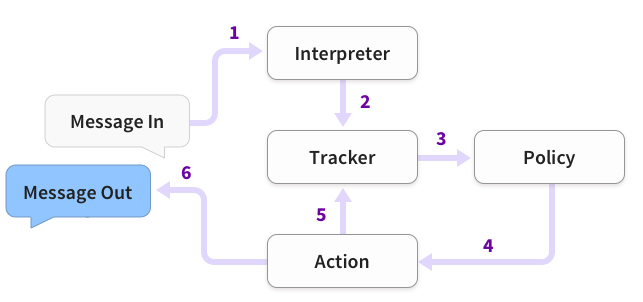
\includegraphics[scale=0.35]{rasa_nlu.png}
	\caption{ Overview of RASA Components }
	\label{fig:ex1}
\end{figure}

Now our main focus in the developmental stage was to map out different intents with examples of how a user might phrase the question. For example, if we had the intent: querying Wikipedia for player information, we would then need specific examples of that intent such as “who is Kyrie Irving”, or “Kyrie Irving”, and place all of those values into a markdown file to use later in the training phase. Furthermore, we may define entities, such as player, team, conference, greeting, and more, and specify those entities in different intents in that same markdown file. So now the example of “who is Kyrie Irving” now becomes “who is [Kyrie Irving](player)”, where the square bracket notation is an example of the player entity. This helps the NLU training policy extract entities from a user's input. After populating an intent with multiple examples of entities (we used the NER\_CRF entity extractor), we were able to train the NLU component (both unsupervised and supervised) and run the interpreter to ensure the intent extraction was performing well enough to start training the dialogue portion of the project. 

\begin{figure}[!htb]
	\centering
	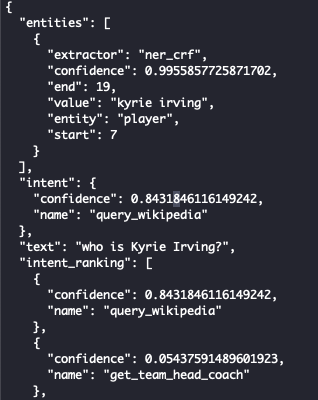
\includegraphics[scale=0.60]{nlu_example.png}
	\caption{ Interpreter returning JSON output }
	\label{fig:ex2}
\end{figure}

As we can see in Figure~\ref{fig:ex2}, when the user inputs “who is Kyrie Irving”, we get a JSON formatted dictionary containing entities, intent, the user's text input, and an intent ranking. First, we can see that the NER\_CRF entities extractor correctly extracted the entity "player" and associated that with the value "Kyrie Irving". Further down in the output, we can see the intent ranking key with a list of confidence and specific intent mappings, where the text input "who is Kyrie Irving" was correctly associated with the intent of querying the Wikipedia API with a confidence rating of 84\%. It's also important to note that we decided on a confidence threshold of 60\% or better before taking a non-text, custom action (i.e. if the user's input was "hello" or some form of greeting, we would reply with a text response instead of defining an action class in Python.)

Once we populated the chatbot domain with more intents, such as finding out when a team plays their next game, getting the eastern conference standing information, etc., and intent/entities extraction was above our confidence threshold, we started the development on the dialogue management component. Here, we used the RASA core engine, and now needed to create a markdown file of "stories", which essentially tells the dialogue model how to behave by defining possible flows of conversation. This is a very powerful feature, as there can be missing "slots" in a user's input that are needed in order to take some sort of action. For example, if the user wanted to information about a player, but didn't specify which player, the chatbot would need to ask the user for the player's name (the slot) before proceeding. Once the dialogue system is built up, we can assign an intent with either an "utterance", which is a pre-formatted response (usually text, but can include thing such as images), or a custom action defined in Python. In order to define custom actions, we need to make use of the Tracker [4] object as seen in Figure~\ref{fig:ex1}, which keeps track of conversation state, receiving the information from a new user message. We needed this Tracker object is order to get the user's last text input or the associated intent of that input in order to use the objects in the NBA\_api library.

\section*{Results}
Currently, the chatbot is able to do a couple of things fairly well. For starters, we were able to implement many different intents in the chatbot's domain. When the training stage ended, our model was able to correctly identify these intents with a confidence rating above our threshold, which was exciting. When a user asked a question where the entity wasn't specified in the domain, it was still able to determine the intent correctly after both supervised and unsupervised training. Additionally, the chatbot was able to run the correct action associated with the user's intent. The problems that arose during development were more geared towards configuring the response back to the user, rather than the overall infrastructure of the chatbot.

\section*{Discussions}
In the introduction section, we defined a hypothesis for this project: if we .... Most of the work in this project was dedicated to looking at RASA's source code and following both online and RASA's documentation tutorials. Unfortunately, both of the tutorials in the documentation for the core and NLU engines, were fairly outdated, making it difficult to follow and piece together. On top of that, the tutorials were of rather simple examples and didn't expand on how to utilize their engines to create something more complex. Following the version history of the RASA framework, it's clear that they're always releasing new versions and drastically change how they format training data and the chatbot domain data. Most of the downfalls in this project can be attributed to either poor decisions made in the early developmental process or us needing more time in order to become more comfortable with the libraries used to help generate a response to the user.

In the project proposal, we intended to use this Python library called "NBA\_py" [5], which configured the stats.nba.com endpoint and returned that information in different formats (JSON, panda arrays, and more.) When it came to the developmental stage of defining our custom actions to take, we didn't realize that the GET requests from this API would mainly result in hanging (never timing out) requests. This was clearly problematic as the library was well managed until the summer of 2017, but since that time period, it was poorly maintained. In conjunction with that time period, the NBA started changing their internal API and the NBA\_py endpoints weren't updated accordingly. We then needed to amend our design decisions, and find another Python library that handled these endpoint configurations or risk doing them ourselves, which would prove to be too time-consuming. After finding another Python library called "NBA\_api", [6] we were able to resume the implementation of these custom actions. At the time this project was due, we were able to get JSON information back from the stats.nba.com, and return that block of JSON back to the user, but failed to parse the JSON correctly and output a more appropriate response.

On another note, we planned on hosting our chatbot infrastructure on Facebook Messenger, allowing the user to interact with the chatbot in a more polished interface. We were able to correctly construct the webhook to the Facebook Messenger API using a Node.js application, and get the user's text input when they sent a message to the chatbot on Facebook Messenger. The problem was that we needed to find a way to return the chatbot's response to the user's question back to the web-hook, but weren't able to find a way for the Python and Node.js programs to communicate with one another. We felt as though this was an important feature to implement as now the chatbot is able to interact with users around the world and therefore would encounter different inputs than what we might have asked it during the testing phase.

\section*{Improvements}
For the future, we could implement many different features that could expand the capabilities of this chatbot, allowing it to interact with the user more fluidly. First, before implementing any new intents, we would need to get more comfortable with the NBA\_api, which would allow us to use the internal methods that formatted the data in a way that we could use. After parsing that JSON, we could extract the information we needed, and return to the user the information that they requested, making the chatbot have an actual use. After that, we could continue implementing new intents, while continuing training our models to handle user input that's not yet specified in its domain.

Another big feature we would eventually like to implement is finding a way for the Python application to communicate with our Facebook Messenger page. Additionally, once that it's implemented, we would also need to host our application on a server or instantiating an EC2 instance on Amazon Web Services, instead of hosting it locally using ngrok [7] application. 

The interaction between the software and user should flow naturally, similar to other artificial intelligence systems, such as Alexa, Siri, or Google Voice Assistant. With a firm foundation, we would expand the variety of functionality. Similar to querying past NBA statistics, a query of predictions could be possible. With past player data, such as points, shooting percentages, playing minutes, it is very much possible to train a logistical model that could predict future stats. Another expansion would be querying dates for future games that could be relayed to the user at the appropriate times. This could translate to being imported into a portable application on the phone in the future. For the project, it was meant to run on the terminal. Hosting on a social media site such as Facebook would have been appropriate to show off during the presentation, but in the future for any alpha beta releases, a release of a compact form of phone application is ideal. Additionally, to fully emulate an artificial intelligence system like Alexa, Siri, or the Google Virtual Assistant, we could also add the ability to communicate with the chatbot verbally, implementing this feature using pre-existing voice-to-text software and dumping that text input into either stdin in the terminal or whatever medium we decide is applicable.

\section*{Conclusion}
Our task was to create a chatbot that interacts with the user in a closed-domain environment, returning relevant NBA information based on the user's input and correctly identifying the intent or context of that input. Most of our effect during this project was looking through RASA AI framework and the different NBA Python libraries that were used at some point during this project. While moving towards using the full RASA AI framework proved to be a good adaption in the development process, due to its vast capabilities and abstraction of NLP techniques, this meant dedicating most of our effort towards reading the source code of RASA and figuring out how to best use its components. This, in turn, took away time that could have been dedicated to working with the NBA\_api and having a more polished response from the output of the custom actions back to the user. 

Overall, we were able to successfully create the foundation of this chatbot, while still allowing room to grow in adding more features, such as expanding the list of defined intents. We were unsuccessful in returning structured responses back to the user and needed more time in order to fully understand the NBA\_api library and the Tracker and Domain objects in RASA. In further releases, we specified some of the things that we want to tackle in the improvements section, most importantly interacting with this chatbot in a different medium, like Facebook Messenger or a mobile application.

\section*{Acknowledgment}
The work described in this paper was conducted as part of a Fall 2018 Artificial Intelligence course, taught in the Computer Science department of the University of Massachusetts Lowell by Prof. Jonathon Mwaura.


\section*{References}
[1] 	“Rasa Stack: Open source conversational AI,” Rasa. [Online]. Available: https://rasa.com/products/rasa-stack. [Accessed: 20-Dec-2018].

[2] 	“Natural Language Toolkit,” NLTK Book. [Online]. Available: https://www.nltk.org/. [Accessed: 20-Dec-2018].

[3] 	“Training and Policies,” Rasa. [Online]. Available: https://rasa.com/docs/core/policies/. [Accessed: 20-Dec-2018].

[4] 	RASA, “High-Level Architecture of RASA framework,” Rasa. [Online]. Available: https://rasa.com/docs/core/0.12.3/architecture/. [Accessed: 20-Dec-2018].

[5] 	Swar, “NBA Python API,” GitHub, 11-Dec-2018. [Online]. Available: https://github.com/swar/nba\_api. [Accessed: 20-Dec-2018].

[6]	Seemethere, “NBA\_PY API,” GitHub, 28-Jun-2017. [Online]. Available: https://github.com/seemethere/nba\_py. [Accessed: 20-Dec-2018].

[7]	Inconshreveable, “Public URLs for exposing your local web server.,” ngrok - secure introspectable tunnels to localhost. [Online]. Available: https://ngrok.com/. 		   [Accessed: 20-Dec-2018].

\end{document}
